\section{Graph Representations}\label{ss_4_graph_repr}

As we have re-iterated several times, an important goal of studying graph structure is to \texttt{(1)} classify nodes \texttt{(2)} predict existence of links \texttt{(3)} classify (sub)graphs. In this chapter we explore mostly unsupervised ways of performing these tasks. A primary characteristic of graph data is that the data is ``simple" but well-structured, compared to typical deep learning problems where each sample is feature rich individually but independent from all other samples. For example, for computer vision tasks, each image itself contains thousands or millions of pixels (e.g. $128 \times 128=16,384$ pixels, like ImageNet \href{http://image-net.org/explore}{[link]}). In comparison, with a movie recommendation dataset, all we have are user ID, their watched movies and movie properties, which are essentially large tables made of a few columns (like \textit{The Movies Dataset} hosted by Kaggle \href{https://www.kaggle.com/rounakbanik/the-movies-dataset}{[link]}). 

{
\centering
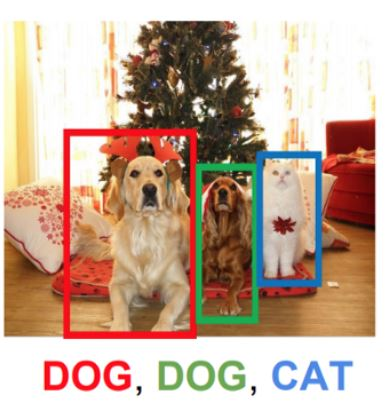
\includegraphics[width=0.3\linewidth]{notes/img/n4_image_classification.JPG} 
\hspace{2cm}
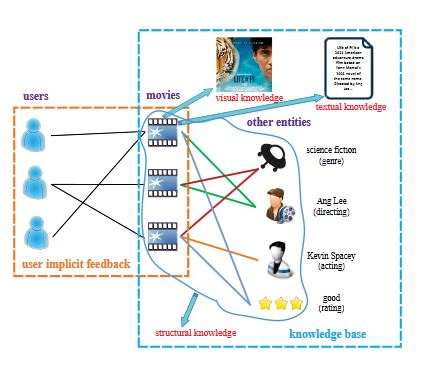
\includegraphics[width=0.4\linewidth]{notes/img/n1_movies.jpg} \par
}

This approach differs from previous influence spread/belief propagation approach. Previous methods are statistical in nature, leveraging heavily knowledge related to Bayesian networks (those that you will learn in CS228). This chapter primarily focuses on, as the section title suggest, learning a graph representation in the form of an embedding that represent graph and its components in the latent space. We will be exploring methods to generate node embedding and graph embedding in the following sections.

\subsection{Node Embedding}

Generating embedding for nodes is analogus to generating word embeddings as part of a natural language processing task. Node with similar embeddings represent similar objects, much like words with similar embeddings have similar semantic meanings. Researchers evaluate embedding similarities in L1-distance, L2-distance (or Forbenius norm), and cosine-distance. Graph applications often choose cosine distance whereas CV/NLP tasks are less biased on the selection of similarity functions.

Putting it in simple terms, we want to encode nodes so that similarity in the embedding space approximates similarity in the original network. We will be defining what \texttt{(1)} encoding function \texttt{(2)} similarity function \texttt{(3)} neighbor definition \texttt{(4)} optimization function now.

{
\centering
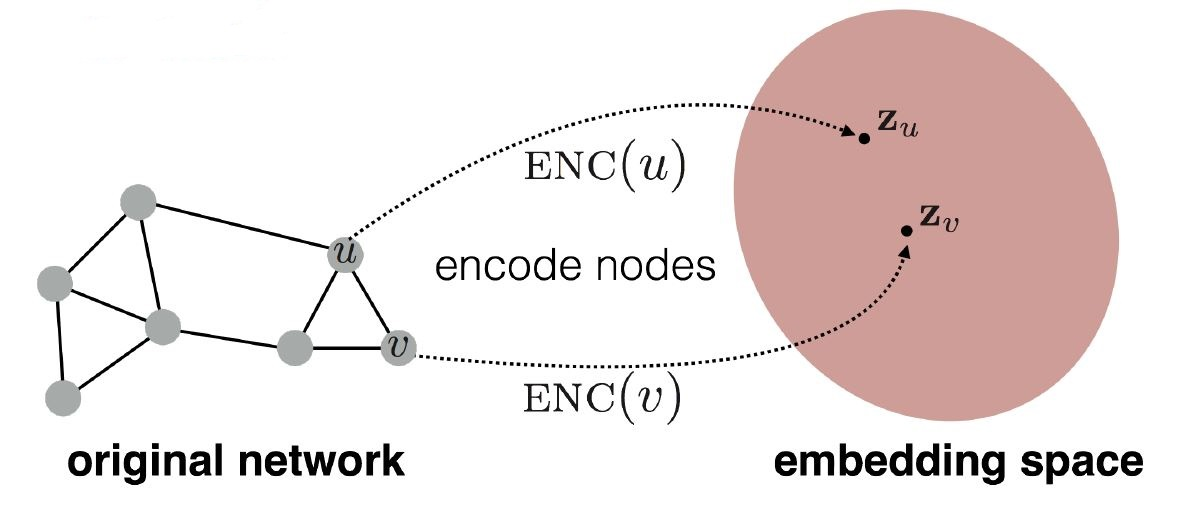
\includegraphics[width=0.65\linewidth]{notes/img/l7_p12_embedding.JPG} \par
}

\subsubsection{Some Basic Ideas}

\paragraph{Embedding lookup} is rather simple. For a graph $G(V, E)$, a node can be represented by a one-hot indicator vector $v \in \mathcal{R}^{|V|}$, and $d$-dimensional embeddings are stored in a lookup matrix $Z \in \mathcal{R}^{d \times |V|}$. Common methods to generate the embedding matrix include DeepWalk, node2vec and TransE, all of which will be covered in later sections of the note.

\begin{align}
    ENC(V_i) &= \mathbf{Z}v_i
\end{align}


\paragraph{Node similarity} can defined in a number of ways, depending on how we want to discover/evaluate node similarity. Here, we use cosine similarity to evaluate node similarity. Recall that

\begin{align}
    \vec{a} \cdot \vec{b} &= |a||b|cos(\theta)
\end{align}

Node similarity in terms of cosine similarity can simply be expressed as  the following. And of course, other similarity functions can also be employed, with appropriate change to optimization function that we will be discussing later (mostly in terms of taking derivative to minimize log-likelihood).

\begin{align}
    similarity (u, v) &= \mathbf{Z}_u \cdot \mathbf{Z}_v \\
                      &= \mathbf{Z}_u^T \mathbf{Z}_v
\end{align}{}

\subsubsection{Random Walk}

Here we are primarily dealing with one large graph, while the same argument applies to a number of smaller graphs as well with appropriately assigned weights to a series of smaller graphs.

Random walk is the most similar to observing sentences for a language modeling task. Imagine we convert all sentences into a large graph where graph neighbours are defined as words that are immediately next to each other, a walk along these paths should form sentence-like samples (or backwards, but backwards sentences are still useful for bi-directional recurrent models). For these language models, researchers define an \textit{n-gram} (or \textit{Skipgram}, depending on the setup) model that tracks probabilities of word co-occurance. See \href{https://web.stanford.edu/~jurafsky/slp3/3.pdf}{[here]} for Prof. Dan Jurafsky's note on \textit{N-Grams}.

{
\centering
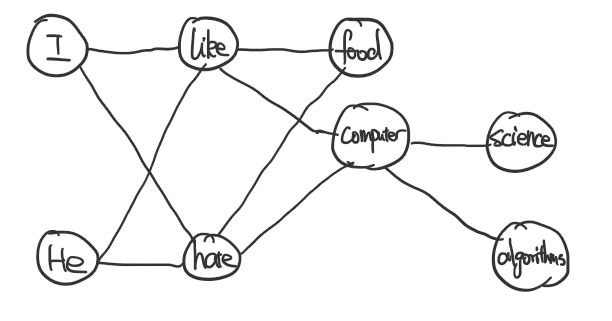
\includegraphics[width=0.65\linewidth]{notes/img/n4_sentences.JPG} \par
}

For random walk in a defined graph structure starting from node $v$, the walk consists of nodes randomly selected from neighbours of the current head. Every time a head is selected, we move to the head then use neighours of this new head as candidates for the next move. You can view this as sampling from all potential ``sentences", compared to NLP tasks where you are given many possible sentences. After sampling by random walk, similar to \textit{N-Gram}/\textit{Skipgram}, we want to find node co-occurance probabilities and match them with cosine distances between node pairs through optimizing log-likelihood.

{
\centering
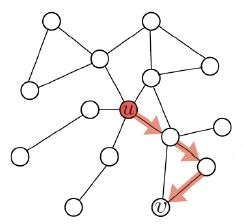
\includegraphics[width=0.4\linewidth]{notes/img/l7_p23_random_walk.JPG} \par
}

Primary benefits for random walk is the following

\begin{itemize}
    \item \textbf{Expressivity}: Walking distance and similarity function together allow incorporation of local and higher-order neighbourhood information
    
    \item \textbf{Efficiency}: Do no need to consider all node pairs and random selection is naturally weighted.
\end{itemize}{}

More formally, given graph $G=(V, E)$, embedding matrix to be optimized $\mathbf{Z} \in \mathcal{R}^{d \time |V|}$, neighbor (as defined in lecture) function $N_R(v)$ as set of nodes visited in a random walk following strategy $R$ and probability function $P$ which is really just proportional to the node similarity function. Likelihood and negative log-likelihood can be defined as the following

\begin{align}
    \mathcal{L} &= \Prod_{u \in V}P(N_R(u) | z_u) \\
    log \mathcal{L} &= \sum_{u \in V}log P(N_R(u) | z_u) \\
                    &= \sum_{u \in V}\sum_{v \in N_R(u)}log P(\mathbf{Z}_v | \mathbf{Z}_u) \\
    \intertext{\qquad \qquad Then for maximum negative log-likelihood}
                &\rightarrow \max_{\mathbf{Z}} \sum_{u \in V}\sum_{v \in N_R(u)}-log P(\mathbf{Z}_v | \mathbf{Z}_u)
    \intertext{\qquad \qquad Here, we define $P(\mathbf{Z}_v | \mathbf{Z}_u)$ as }
    P(\mathbf{Z}_v | \mathbf{Z}_u) &= \frac{exp(\mathbf{Z}_v^T\mathbf{Z}_u)}{\sum_{n \in V}exp(\mathbf{Z}_n^T\mathbf{Z}_u)} \\
    log \mathcal{L} &= \sum_{u \in V}\sum_{v \in N_R(u)}log \frac{exp(\mathbf{Z}_v^T\mathbf{Z}_u)}{\sum_{n \in V}exp(\mathbf{Z}_n^T\mathbf{Z}_u)}
\end{align}{}

We observe that denominator $\sum_{n \in V}exp(\mathbf{Z}_n^T\mathbf{Z}_u)$ have to be computed for all $v \in V$, resulting in $O(n^2)$ complexity. One way to alleviate this problem is simply sub-sample from $V$ when computing the denominator sum. We could use ``negative sampling" as used for \textit{word2vec} explained \href{https://arxiv.org/pdf/1402.3722.pdf}{[here]}. Here, ``positive" means nodes that are in $N_R(u)$ in any of the walks we performed, and ``negative" means all other nodes not visited from walks initiated from $u$. Observe the following expression. We are \texttt{(1) } maximizing $exp(\mathbf{Z}_v^T\mathbf{Z}_u)$ and minimizing sum of similarities from negative samples. ($exp$ is used here instead of $\sigma$ for sigmoid, for simplicity, the same result is achieved regardless). This way, we are minimizing the probability of a random node having high similarity with the source node. Number of negative samples (k) is typically $5-20$, depending on the application and degree of vertices in the graph. The random walks are often fixed length without preventing repeats, like \textit{DeepWalk} implementation \href{https://arxiv.org/pdf/1403.6652.pdf}{[link]}. This paper contains pseudocode and more formal work on random walk and \textit{skipgram}. For a more intuitive explanation on \textit{hierarchical softmax}, which is not immediately relevant in this context, can be found \href{https://www.quora.com/What-is-hierarchical-softmax?share=1}{[here]}.

\begin{align}
    log \frac{exp(\mathbf{Z}_v^T\mathbf{Z}_u)}{\sum_{n \in V}exp(\mathbf{Z}_n^T\mathbf{Z}_u)} &= log(exp(\mathbf{Z}_v^T\mathbf{Z}_u)) - \sum_{n \in neg\_sampling(V, walks)}exp(\mathbf{Z}_n^T\mathbf{Z}_u)
\end{align}{}

\paragraph{Biased random walk} is a random walk with a predefined node selection probability. \textit{node2vec} proposes a wal strategy that balances exploration of local neighborhood and going further out. As shown below, $S_2$ is the same ``level" as $W$, whereas $S_3$ is further out. We assign different probabilities to $S_2\ versus\ S_3, S_4$. That is, there is $\propto 2/q$ chance of going further, $\propto 1/p$ chance of returning to $S_1$ and $\propto c$ chance of going to $S_2$. (Values shown in labels need to be normalized).

{
\centering
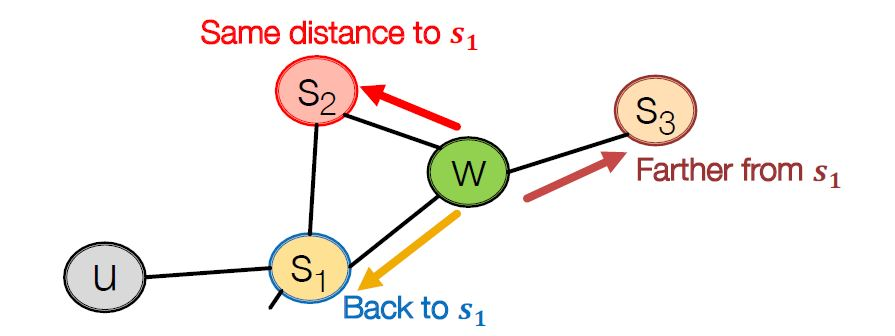
\includegraphics[width=0.45\linewidth]{notes/img/l7_p41_bias1.JPG}
\hspace{1cm}
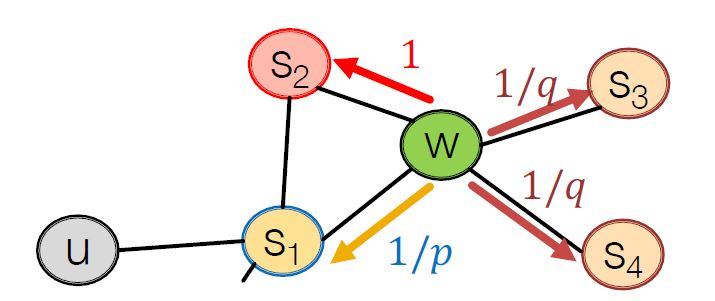
\includegraphics[width=0.45\linewidth]{notes/img/l7_p41_bias2.JPG} \par
}

This is only a different strategy of defining random walk preference ($N_R(v)$). The same gradient descent method for maximizing negative log-likelihood still applies.

We will cover \textit{TransE} later in the notes because it falls in the more ``neural" approach compared to the above more traditional approach.

\subsection{Graph Embedding}

Graph(sub-graph) embedding involves transforming embedding of nodes into one embedding for the entire (sub)graph. Typical embedding `joint" methods include 

\begin{itemize}
    \item Concatenation
    
    \item Hadamard (element-wise product)
    
    \item Sum/Avg (element-wise sum/average)
    
    \item Distance (distance between embeddings with some distance function suitable for $2$ or more vectors)
\end{itemize}{}

There are clearly more effective methods than the above embedding joining methods that lead to higher quality graph-level embeddings.

\subsubsection{Naive Concatenation}

As said, we just naively run some node embedding algorithm (neural or traditional), then average all node embeddings \href{https://arxiv.org/pdf/1509.09292.pdf}{[link]}. This is the most robust as embeddings will have fixed length and not blow up/vanish in scale if sum or product is taken. 

\subsubsection{Virtual Node}

Instead of averaging embeddings, we create a virtual node that connects to the entire graph (or relevant nodes only, for sub-graph) then compute embedding for the virtual node. Analogy of this is creating a source/sink pair when we are transforming difficult graph problems to max flow min cut problems that have well-known fast-ish solution. See the publication \href{https://arxiv.org/abs/1511.05493}{[here]}.

\subsubsection{Anonymous Walk}

Anonymous walk is a fancy name of saying instead of having a $|V|$ size one-hot vector, we only use a size $k$ one-hot vector for a $k$-length random walk. That is, we only care about whether a different node has been visited in a walk, rather than the actual identity of the node. 

{
\centering
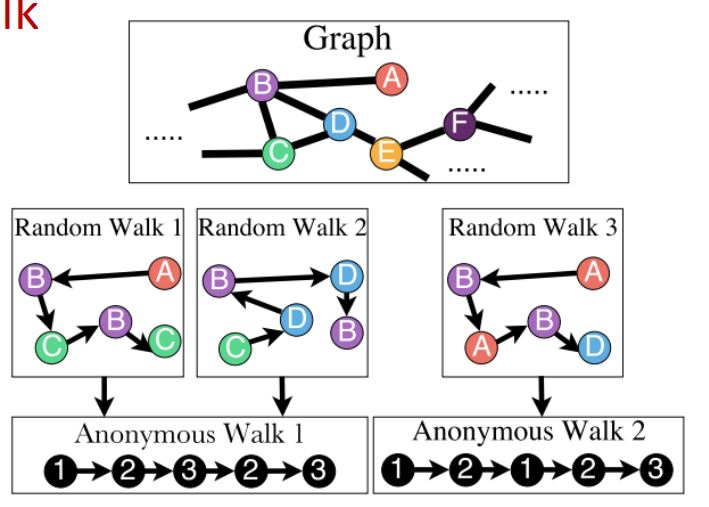
\includegraphics[width=0.55\linewidth]{notes/img/l7_p58_anonymous.JPG} \par
}

As expected, total number of different $k$-length grows as $k$ increases. In fact, it should grow proportionally (but faster than) to $\frac{k^k}{p!}$ (think about how many, allowing repeats, different combinations can exist). This estimate is NOT accurate because it over-penalizes low $k$ scenarios. The growth chart below reflect the true number of anonymous walks. The approximation ratio grows (or shrinks, depends on how you define approximation ratio) at approximately $2$.

{
\centering
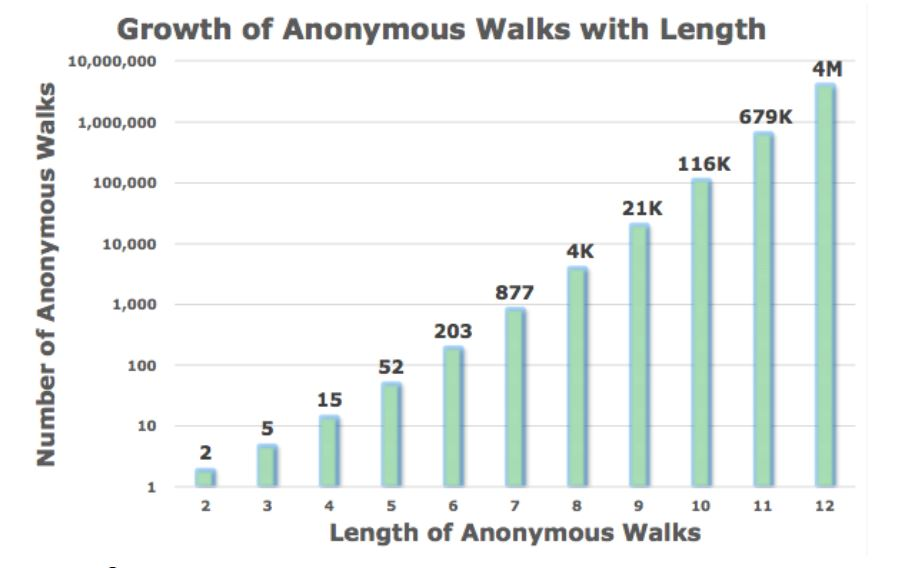
\includegraphics[width=0.55\linewidth]{notes/img/l7_p59_count.JPG} \par
}

\paragraph{Idea 1, enumerate all walks} We define $d$ as number of distinct random walks for length-$k$ walks. Then each $\mathbf{Z}_v^{i}$ is the probability of obtaining the i-th anonymous walk starting the walk at node $v$. Without considering weight associated with bias, we can enumerate all possible walk paths then for each node, we compute the probability of obtaining the $i$-th anonymous walk starting at node $v$.

\paragraph{Idea 2, sample and deal with sampling error} We can obtain the previous probability by sampling a large number of random walks then process for each node. Here we use some statistical trick to argue that to obtain error of no more than $\epsilon$ with probability less than $\delta$, we need to sample

\begin{align}
    m = \Big[\frac{2}{\epsilon^2}(log(2^\eta - 2) - log(\delta))\Big] \comment{where\ $\eta$ is number of different anonymous walks for $k$-length walk}
\end{align}{}

\begin{todo}
    I suspect this is derived from multiplicative form of Chernoff bound. Wikipedia page for Chernoff bound is not a bad place to start \href{https://en.wikipedia.org/wiki/Chernoff_bound}{[link]}.
\end{todo}{}

\paragraph{Idea 3, use Skipgram again} Notice that the above ``dumb" methods are what NLP researchers used to create language model. \textbf{Idea 2} is not much different for the argument that negative sampling reaches approximately the same error, if you spent the time of digging all the formalities out. Therefore, \textbf{Idea 3} is simply treat each anonymous walk as a ``token". Suppose from node $v$ we can have anonymous walks $w_1, w_2 \dots w_t$, then as defined for \textit{Skipgram}, we want to maximize $P(w_m | \{w_1, w_2 \dots w_t\} \setminus w_m)$. We are claiming that $N_R(u) = \{w_1, w_2 \dots w_t\}$, re-using the neighborhood notation we user earlier for node embedding. All other expressions for \textit{Skipgram} applies and we want to maximize, as in lecture

\begin{align}
    max \frac{1}{T}\sum_{t=\delta}^{T}log P(w_t|w_{t-\delta}, \dots w_{t-1})\\
    P(w_t|w_{t-\delta}, \dots w_{t-1}) &= \frac{exp(y(w_t))}{\sum_i^{\eta} exp(y(w_i))} \\
    y(w_t) &= b + U \cdot (\frac{1}{\delta}\sum_{i=1}^{\delta}v_i)
\end{align}{}

Formal derivation of this part of the notes is discussed in the \textit{Anonymous Walk Embedding} paper \href{https://arxiv.org/pdf/1805.11921.pdf}{[link]}.


\section{Neural Model for Graphs}

In the previous section, we discussed traditional methods of generating embeddings for node and graphs. In this section, we move on to neural models that started gaining tracking only in recent years (approximately 2013, when the foundational \textit{TransE} paper was published \href{https://papers.nips.cc/paper/5071-translating-embeddings-for-modeling-multi-relational-data.pdf}{[link]}). This progress, viewing it from the perspective of Stanford's AI course offerings, is from CS229 (machine learning) to CS230 (deep learning). In terms of actual methods used, we are moving from \textit{word2vec} and \textit{Skipgram} model to convolutional and recurrent neural networks. For graph related topics, the following content is the neural ``equivalent" for CS228 (probabilistic graphical models).

There are several problems with getting embedding from random walks as shown in Section \ref{ss_4_graph_repr}. \texttt{(1)} these node embeddings are generated independently (at best locally) from each other (remember that we are only approximating the log-likelihood) \texttt{(2)} we cannot generate node embedding for future nodes, which means the graph itself is pre-determined, \texttt{(3)} the incorporation of local/macro level structure is questionable despite us playing with biased random walk while leaving structure of the graph itself on the table.

Applying existing models like convolutional neural network and recurrent neural network sounds problematic because they are designed for samples that has internal structures, not samples that are well-structured (but not following a fixed pattern) to connect to other samples. For example, in the case of image convolution, we define a $d_1 \times d_2 \times c$ (dim, dim, channel) kernel that scans the image. This is clearly not possible as we cannot define a fixed size ``kernel" for graphs because nodes do not all have the same edge connectivities. 

{
\centering
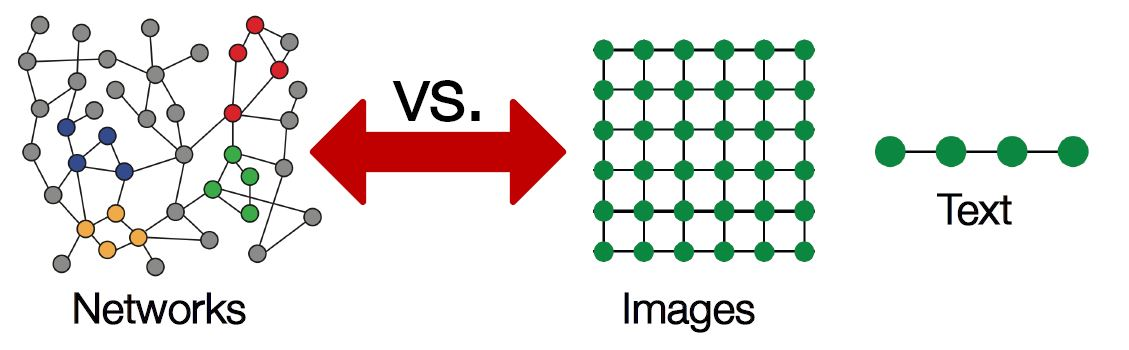
\includegraphics[width=0.75\linewidth]{notes/img/l8_p12_compare.JPG} \par
}

\subsection{Components of Graph Convolution}

Naturally, convolution is a form of recursion where recursion depth is number of layers we include in the convolution. To fully define this ``recursion" we need to figure out \texttt{(1)} what do to with embedding from previous layer? \texttt{(2)} what message is passed from node in the previous layer to the current node \texttt{(3)} how to aggregate messages from previous layer \texttt{(4)} how to aggregate/post-process this aggregated message with embedding of the current node. Putting everything together, for $h_v^k$ as embedding for node $v$ after $k$-th recursion,

\begin{align}
    h_v^k &= \phi(AGG_1\Big[ op_1\big[(AGG_2(\{MSG(u, v), \forall u\in N(v)\})\big], op_2(h_v^{k-1})  \Big])
\end{align}{}

We define the various ``placeholder functions" as the following. I'm sure you can also convert computer vision task to something like this where $h_v^k$ is equivalent to a pixel-level multi-channel vector. 

\begin{itemize}
    \item $\phi \rightarrow$ Activation function for embedding (tanh, softmax, etc.)
    
    \item $AGG_1 \rightarrow$ Aggregation function to join embedding from previous layers and embedding of current node from previous step (concatenation, sum/avg, attention, etc.)
    
    \item $op_1 \rightarrow$ Weight assigned to messages from previous layer after aggregation (typically just a matrix multiply)
    
    \item $AGG_2 \rightarrow$ Aggregation function to join embedding from nodes in the previous layer(concatenation, sum/avg, attention, etc.)
    
    \item $AGG_2 \rightarrow$ Message function to compute message from nodes in the previous layer to current node (depends on whether edge embeddings exist or if we are handling non-existing edges differently)
    
    \item $op_2 \rightarrow$ Weight assigned to embedding of the current node from previous iteration (typically just a matrix multiply)
    
    \item $N \rightarrow$ Neighbour of a node (typically immediate neighbours, but researchers have used other definitions, such as \textit{RippleNet}, \href{https://arxiv.org/pdf/1803.03467.pdf}{[link]})
\end{itemize}

On top of this, of course, there is also embedding initialization methods and loss function for gradient descent. Little generalization can be applied to these functions as they are task dependent.

A comprehensive survey of various graph neural network methods as of 2019 is \href{https://arxiv.org/pdf/1901.00596.pdf}{[here]} and \href{https://arxiv.org/pdf/1812.08434.pdf}{[here, a bit older]}. For this class, we discuss \textit{TransE} (Sec \ref{ss_52_transe}), \textit{TransR} (Sec \ref{ss_53_transr}), \textit{GraphSAGE} (Sec \ref{ss_54_sage}), \textit{PinSage} (Sec \ref{ss_55_pin_sage}) and \textit{GAT} (Sec \ref{ss_56_gat}).

\subsection{TransE, Translating Embeddings for Modeling Multi-relational Data} \label{ss_52_transe}

The foundational TransE implementation was proposed in 2013 \href{https://everest.hds.utc.fr/lib/exe/fetch.php?media=en:cr_paper_nips13.pdf}{[link]}. We reproduce the algorithm (not a screenshot) below. We define $(h, l ,t)$ triplet as (head entity, relation, tail entity), or graphically, $v_h \xrightarrow[]{l} t_h$.

\begin{algorithm}[H]
\SetAlgoLined
%\KwResult{Write here the result }
\textbf{input:} Training set $S=\{h, l, t\}$, entities and rel.sets $E$ and $L$, margin $\gamma$, embeddings dim. $k$. \\
%\hspace*{\algorithmicindent} \textbf{Input:}\\
%\hspace*{\algorithmicindent} \textbf{Output} 
\textbf{initialization} \\
\hspace*{\algorithmicindent} $l = uniform(-\frac{6}{\sqrt{k}}, -\frac{6}{\sqrt{k}}) \qquad  \forall l \in L$ \Comment{$\frac{6}{\sqrt{k}}$ is most likely from Xavier initialization} \\
\hspace*{\algorithmicindent} $l = l / ||l|| \qquad \forall l \in L$ \\
\hspace*{\algorithmicindent} $e = uniform(-\frac{6}{\sqrt{k}}, -\frac{6}{\sqrt{k}}) \qquad \forall e \in E$ \\
\While{Loss not converged}{
    $e = e / ||e|| \qquad \forall e \in E$ \\
    $S_{batch} = rand\_sample(S, b)$ \Comment{sample $b$ triplets from set $S$} \\
    $T_{batch} = \emptyset$ \Comment{Set initial pairs of triplets to be empty} \\
    \For{$(h, l, t) \in S_batch$}{
      $(h', l, t') = rand\_sample(S')$ \Comment{Sample an invalid $(h', l, t')$ triplet (exactly one or two of $h, l, t$ have to be different)} \\
      $T_{batch} = T_{batch} \cup \{((h, l, t), (h', l, t'))\}$
     }
 Gradient descent on $\sum_{((h, l, t), (h', l, t')) \in T_{batch}} \nabla[\gamma + d(h + l, t) - d(h' + l, t')]$
 \caption{Learning \textbf{TransE}}
 }
\end{algorithm}

To explain what this ``sample an invalid triplet" is all about, let's use a visual Q\&A example \href{https://people.cs.vt.edu/sudo777/files/siamese-network-pptx.pdf}{[link]}. With this example, you want to make sure that embedding of an image with \underline{girl} \textit{walking a bike} is different from images \underline{boy} \textit{walking a bike}. So, $h$ is \textit{boy/girl}, $l$ is \textit{walking a bike}, $t$ is the image. We want to make sure that translating \textit{boy/girl} with operator \textit{walking a bike} do NOT land in the same target image. Hopefully this analogy help you understand the rationale behind setting up the gradient update rule. Search for \texit{Siamese network} \href{https://en.wikipedia.org/wiki/Siamese_neural_network}{[link]} for similar setups (commonly used for facial identification).

{
\centering
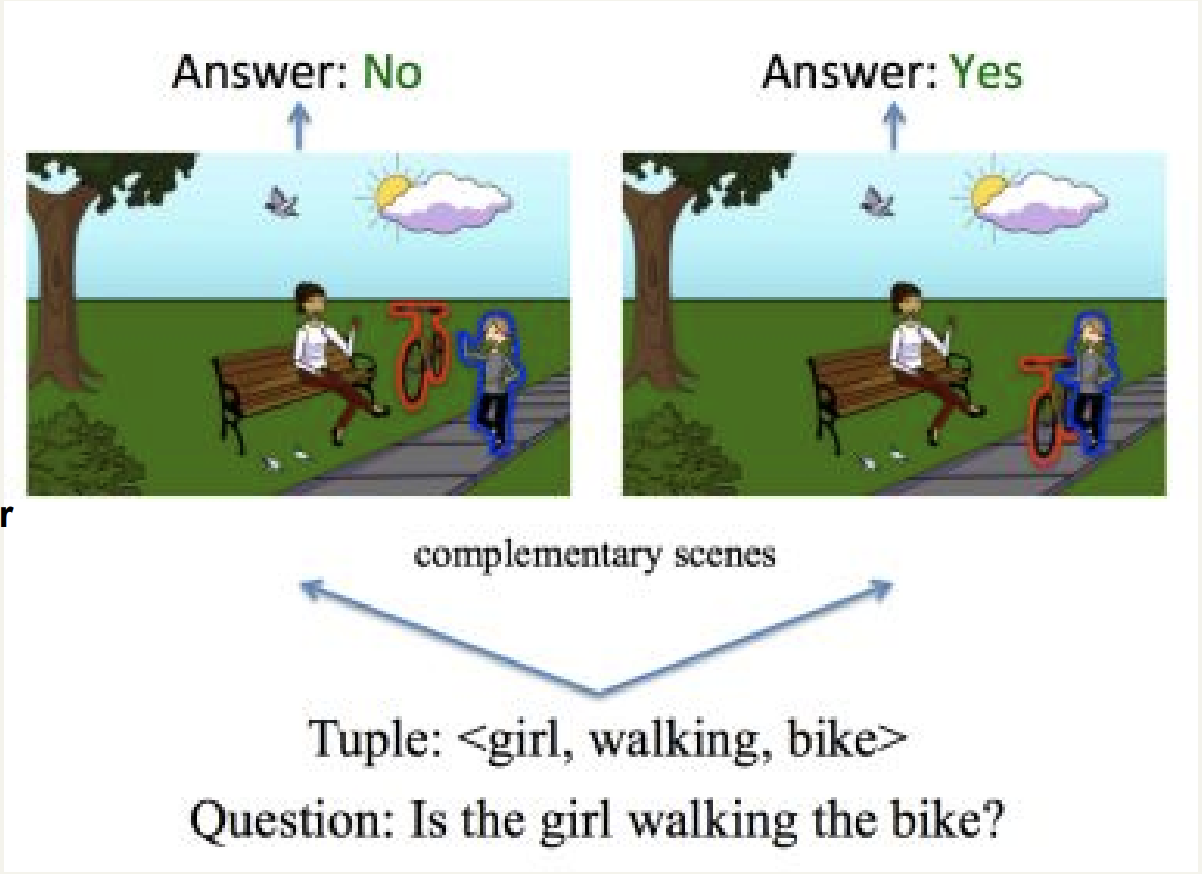
\includegraphics[width=0.6\linewidth]{notes/img/n5_siamese.png} \par
}

\subsection{TransR, Learning Entity and Relation Embeddings for Knowledge Graph Completion} \label{ss_53_transr}

\subsection{GraphSAGE, Inductive Representation Learning on Large Graphs} \label{ss_54_sage}

\subsection{PinSage, Graph Convolutional Neural Networks for Web-Scale Recommender Systems} \label{ss_55_pin_sage}

\subsection{GAT, Graph Attention Networks} \label{ss_56_gat}

